% https://tex.stackexchange.com/questions/51757/how-can-i-use-tikz-to-make-standalone-svg-graphics
\documentclass{standalone}
\usepackage[svgnames]{xcolor} % Enabling colors by their 'svgnames'
\usepackage{tikz}
\usetikzlibrary{calc}
\usepackage{amsmath,amsfonts,amsthm}
\usepackage{physics}

\begin{document}
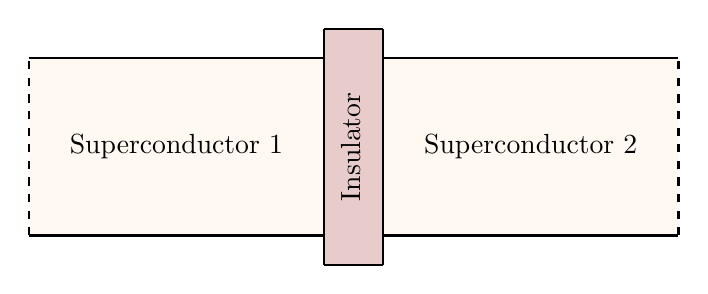
\begin{tikzpicture}[scale=1.5]

    %Coloring
    \fill[color=DarkOrange!5] (0,-0.75) rectangle (2.5,0.75); %Superconductor 1.
    \fill[color=DarkRed!20] (2.5,-1) rectangle (3,1); %Insulator.
    \fill[color=DarkOrange!5] (3,-0.75) rectangle (5.5,0.75); %Superconductor 2
    
    %Superconductor 1
    \draw[thick] (0,0.75) -- (2.5,0.75); %Top line
    \draw[thick] (0,-0.75) -- (2.5,-0.75); %Lower line
    \draw[thick, dashed] (0,-0.75) -- (0,0.75); %Left dashed line
    \node at (1.25,0) {\normalsize Superconductor 1}; %Text
    
    %Insulator
    \draw[thick] (2.5,-1) -- (2.5,1); %Left line
    \draw[thick] (3,-1) -- (3,1); %Right line
    \draw[thick] (2.5,1) -- (3,1); %Top line
    \draw[thick] (2.5,-1) -- (3,-1); %Lower line
    \node[rotate=90] at (2.725,0) {\normalsize Insulator}; %Text
    
    %Superconductor 2
    \draw[thick] (3,0.75) -- (5.5,0.75); %Top line
    \draw[thick] (3,-0.75) -- (5.5,-0.75); %Lower line
    \draw[thick, dashed] (5.5,-0.75) -- (5.5,0.75); %Left dashed line
    \node at (4.25,0) {\normalsize Superconductor 2}; %Text
    
\end{tikzpicture}
\end{document}

